\documentclass{article}
\usepackage{graphicx} % Required for inserting images
\usepackage[section]{placeins}

\title{CS180 Project 3}
\author{Kyle Wong}
\date{October 2023}

\begin{document}

\maketitle

\section{Part 1. Defining Correspondences}
Our goal is to morph the shapes of two images together. 
To do this we first need to select corresponding keypoints for each image. To make a 2d warp we can use a triangular mesh that covers the whole image, using keypoints such that the triangles in each image correspond to each other. A good method for getting more evenly sized triangles is to use Delaunay triangulation to produce the triangular mesh.

\begin{figure}[!htb]
    \centering
    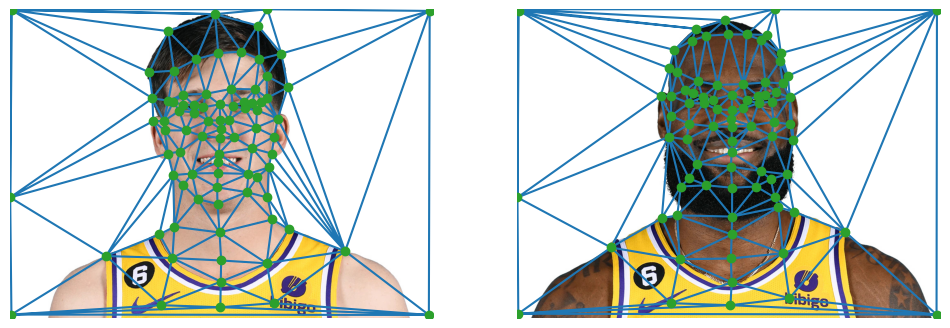
\includegraphics[scale=0.5]{im1.png}
\end{figure}

\section{Part 2. Computing the “Mid-Way Face”}
We must figure out how to get from one triangle to the corresponding triangle in the transformed image. We can set up a system of linear equations to solve for the transformation matrix.

Given a triangle T $(a_x, a_y)$, $(b_x, b_y)$, and $(c_x, c_y)$ and a triangle T' with vertices $(a_x', a_y')$, $(b_x', b_y')$, and $(c_x', c_y')$ we can set up a system of linear equations that describes this affine warp.

\begin{figure}[!htb]
    \centering
    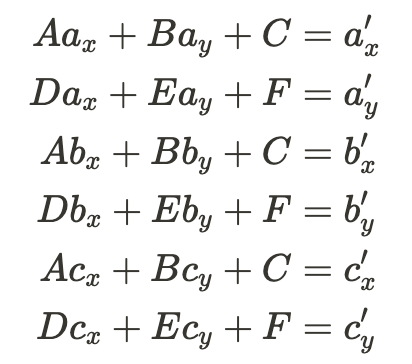
\includegraphics[scale=0.5]{im2.png}
\end{figure}

\begin{figure}[!htb]
    \centering
    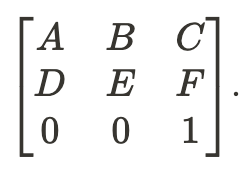
\includegraphics[scale=0.5]{im3.png}
\end{figure}
\newpage
We can solve this for A = \\

Using this method, we can warp each triangle in the average mesh into the corresponding triangle in the original image’s mesh. This tells us which positions in the original image would warp to each pixel of the midway image, and I used linear barycentric interpolation interpolation to get the color for that pixel.

We do this for both of the original face images to get the average shape. To get the average color we average the pixel values and then we have our mid-way face.


\begin{figure}[!htb]
    \centering
    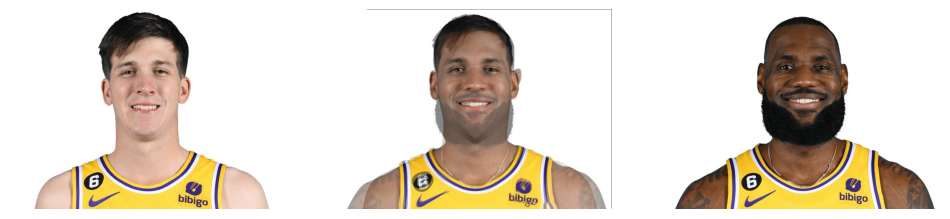
\includegraphics[scale=0.5]{im4.png}
\end{figure}
\newpage


\section{Part 3. The Morph Sequence}
To get each frame of the morph sequence, we perform the same procedure used for generating the mid-way face, but we use a weighted average instead.



\section{Part 4. The “Mean Face” of a Population}
Using The FEI face database (Brazilian face database) dataset, we can compute the average face of this population by calculating the average face shape and morphing each face into the average shape. I did not divide into subpopulations such as gender. Below are some examples of images from the dataset morphed into the average shape for the entire dataset.

\begin{figure}[!htb]
    \centering
    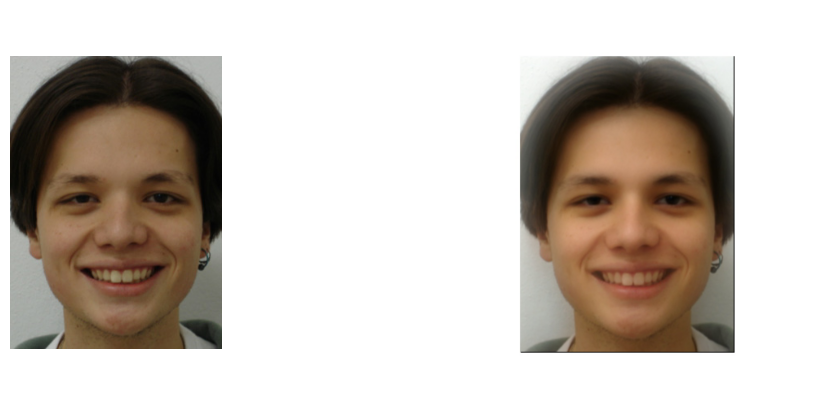
\includegraphics[scale=0.5]{im5.png}
    \caption{Left is the original face. Right is the face morphed into the average shape.}
\end{figure}

\begin{figure}[!htb]
    \centering
    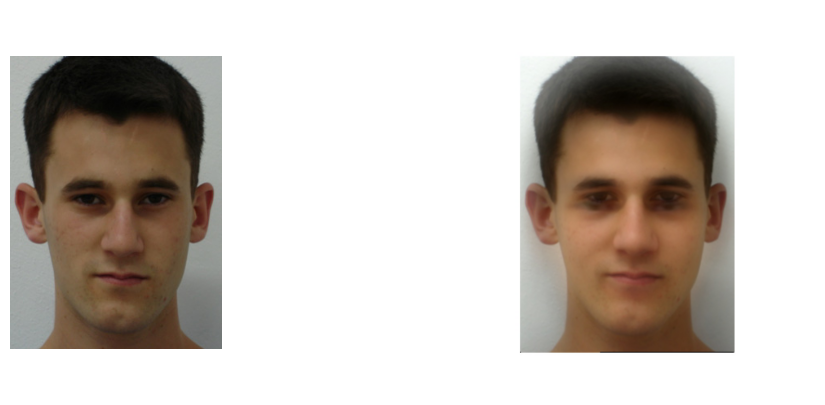
\includegraphics[scale=0.5]{im6.png}
    \caption{Left is the original face. Right is the face morphed into the average shape.}
\end{figure}
\newpage

\begin{figure}[!htb]
    \centering
    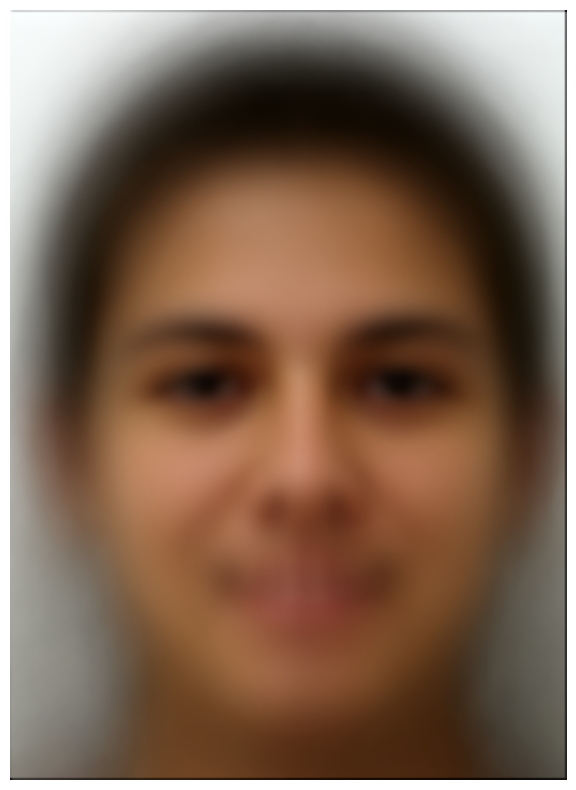
\includegraphics[scale=0.5]{im7.png}
    \caption{Average Face of the Population}
\end{figure}

\begin{figure}[!htb]
    \centering
    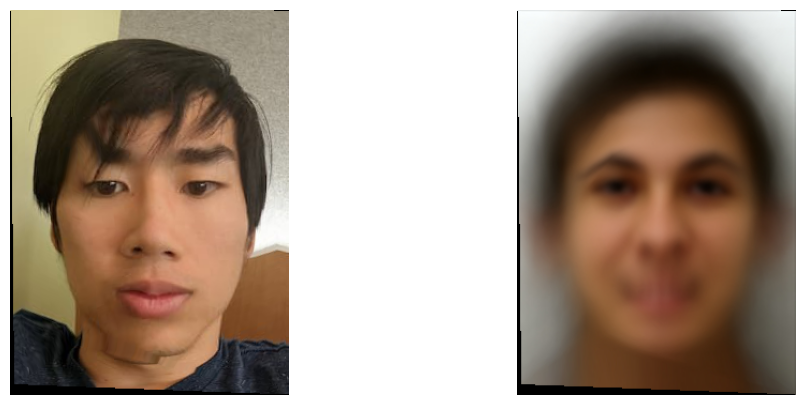
\includegraphics[scale=0.5]{im8.png}
    \caption{Left is my face warped into the average geometry. Right is the average face warped into my geometry.}
\end{figure}
\newpage



\section{Part 5. Caricatures: Extrapolating from the Mean}
Let's consider the average face shape to be a vector h and my face shape to be a vector f, then f$-$h can be interpreted as what is unique about my face and we can extrapolate my face further in those directions. Therefore, by adding $\alpha$(f$-$h) to my face shape (where $\alpha>$0) and morphing my face into the new shape, we can exaggerate my facial features to provide a caricature of myself.

Below are the results for extrapolating from the mean of the entire FEI face database, including males and females.

\begin{figure}[!htb]
    \centering
    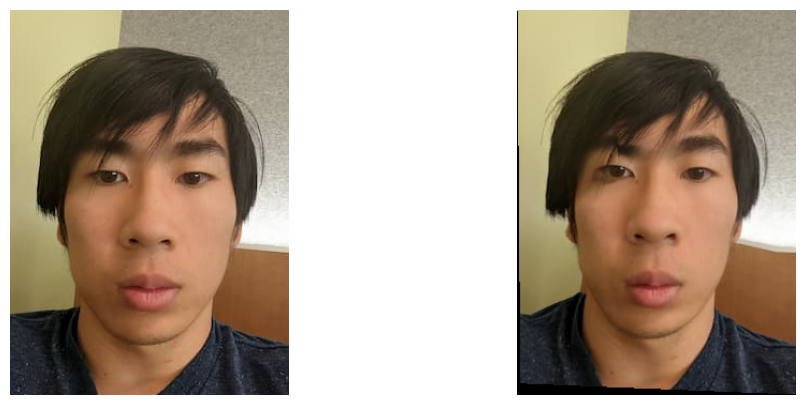
\includegraphics[scale=0.5]{im9.png}
    \caption{Left is my normal face. Right is my face warped onto my unique features with $\alpha$=0.5.}
\end{figure}
\newpage

\section{Bells and Whistles: Change Gender}
Out of curiosity, I projected my face onto the the average shape of Japanese actresses. I also adjusted what the weights accordingly. My correspondence points should have been a little different because it makes my chin really disproportionate. Other than that, I do look better. 

\begin{figure}[!htb]
    \centering
    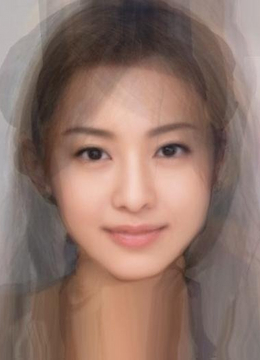
\includegraphics[scale=0.5]{avgjapactress.jpg}
    \caption{Average Japanese actress face}
\end{figure}

\begin{figure}[!htb]
    \centering
    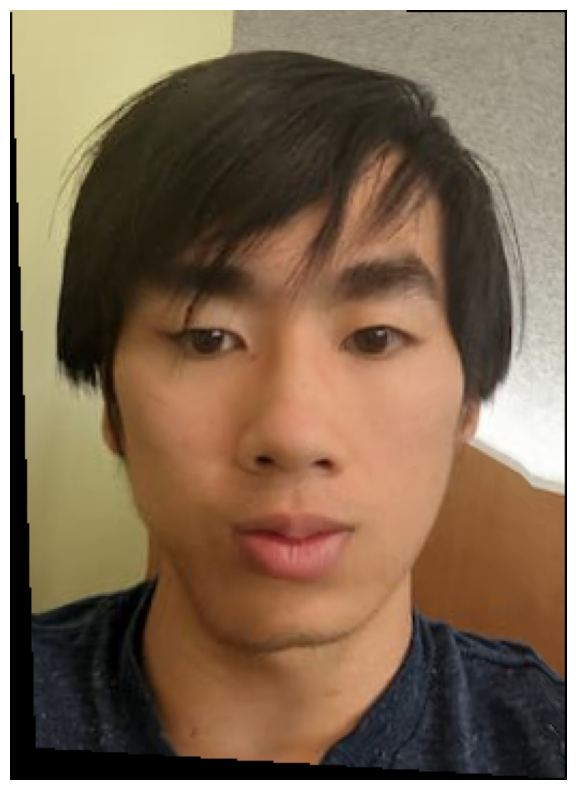
\includegraphics[scale=0.5]{im10.png}
    \caption{Morphing just the shape: My face projected onto the average Japanese actress shape. As you can see my eyes get rounder and my face becomes narrower. My lips are bigger and my nose is a little smaller. So I've become more like typical Asian beauty standards.}
\end{figure}

\begin{figure}[!htb]
    \centering
    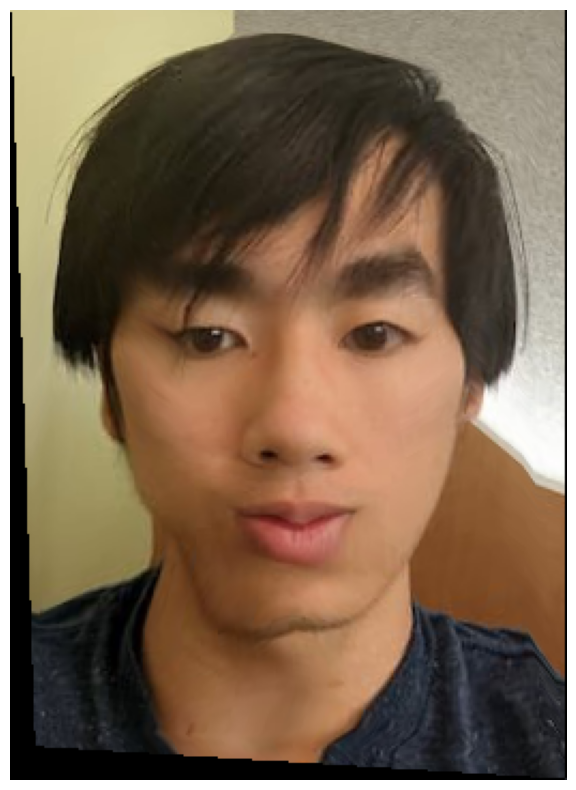
\includegraphics[scale=0.5]{im11.png}
    \caption{I've shifted the weights around and interestingly my face becomes noticeably more disproportionate around my chin. I'm not sure why my chin was so misshapen like that, I'm guessing the correspondence points were a little off.}
\end{figure}

\begin{figure}[!htb]
    \centering
    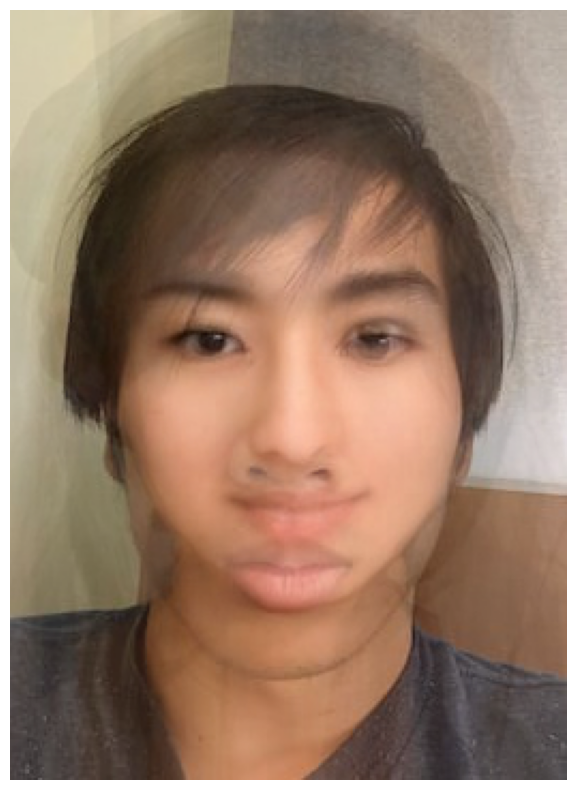
\includegraphics[scale=0.5]{im12.png}
    \caption{Morphing just the appearance: I've averaged the images and it is quite obvious that my photo is misaligned with the average. My face was quite distorted and too close to the camera.}
\end{figure}

\begin{figure}[!htb]
    \centering
    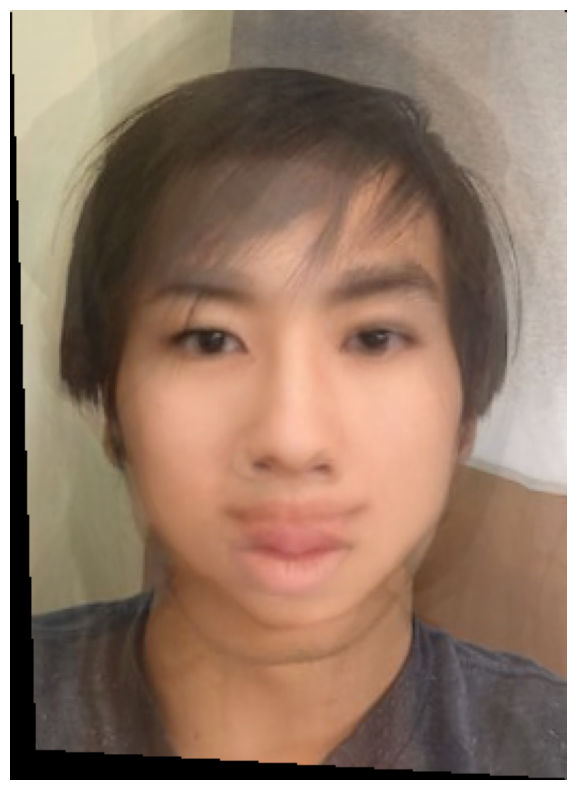
\includegraphics[scale=0.5]{im13.png}
    \caption{Morphing both the shape and the appearance: I've morphed the images together and it seems that I made a mistake with the correspondences so it is slightly misaligned around the mouth and chin.}
\end{figure}
\newpage

\end{document}
